
\documentclass[12pt]{article}

\usepackage[T1]{fontenc}
\usepackage[utf8]{inputenc}
\usepackage[pdftex]{graphicx}
\usepackage{graphics}
%\usepackage{natbib}
\usepackage{amsmath}
\usepackage{siunitx}
\usepackage{epstopdf}
\usepackage[english]{babel}
\usepackage{lmodern}
\usepackage{isotope}
\usepackage{listings}
\usepackage{chngcntr}
\usepackage{subcaption}
%\usepackage[square,numbers]{natbib}
%\bibliographystyle{ksfh_nat}

\counterwithin{figure}{section}
\def\thickhrulefill{\leavevmode \leaders \hrule height 1pt\hfill \kern \z@}

\usepackage{hyperref}
\usepackage{color}
\definecolor{codegreen}{rgb}{0,0.6,0}
\definecolor{codegray}{rgb}{0.5,0.5,0.5}
\definecolor{codepurple}{rgb}{0.58,0,0.82}
\definecolor{backcolour}{rgb}{0.95,0.95,0.92}

\lstdefinestyle{mystyle}{
	backgroundcolor=\color{backcolour},   
	commentstyle=\color{codegreen},
	keywordstyle=\color{magenta},
	numberstyle=\tiny\color{codegray},
	stringstyle=\color{codepurple},
	basicstyle=\footnotesize,
	breakatwhitespace=false,         
	breaklines=true,                 
	captionpos=b,                    
	keepspaces=true,                 
	numbers=left,                    
	numbersep=5pt,                  
	showspaces=false,                
	showstringspaces=false,
	showtabs=false,                  
	tabsize=2
}

\lstset{style=mystyle}
\begin{document}

\begin{figure}
\begin{minipage}{0.5\linewidth}
\begin{flushleft}
\includegraphics[width=5cm]{pics/ethlogo_black.eps}
\end{flushleft}
\end{minipage}
\hspace{0.05cm}
\begin{minipage}{0.5\linewidth}
\begin{flushright}
Manual number:\hspace{2cm}\\[0.5cm]
\includegraphics[width=4cm]{pics/VP-Logo.eps}
\end{flushright}
\end{minipage}
\hrule height 1pt\hfill \\[3cm]
\end{figure} 

\title{Drift Chamber\\ Instructions}
\author{D. Hits, G. Guyer, M. Setz}
\date{rev. D. Hits, \today}
\maketitle

\newpage
\section{Introduction}


This manual contains only a brief introduction to the processes occurring in a drift chamber.In order to gain more complete understanding of the physics of the drift chamber a references at the end of this manual should be consulted \cite{DriftChamberBook, knoll, NIMwiki}. 

Drift chambers belong to the most important measurement devices of nuclear and particle physics. They are a central aspect of nearly every large experiment in high energy physics. In this experiment a small drift chamber is operated and characterized. After that the trajectories of particles from the cosmic radiation should be reconstructed. 

If a charged particle travels through a gas volume, it leaves a trail of ionized gas atoms and free electrons behind. By applying an electric field the ions and electrons can be separated and generate an electric signal. This signal, however, is very small. A high-energy particle with an elementary charge produces only about 100 electron/ion-pairs by going through one centimeter of air. Single particles are therefore only detectable after amplifying this signal. 

In a detector filled with gas there is a simple way to amplify the signal inside the detector, even before it is measured on the outside. If the electric field is sufficiently strong, the free electrons can be accelerated to the energies large enough to ionize gas atoms and create and avalanche which will result in an electric signal many times higher than the original one. The required electric field strengths are easily generated around very thin wires. By using very thin signal wires, one can therefore easily create a detectable signal. Hence already a simple structure allows the detection of particle radiation. Many detectors are based on this principle, from a simple Geiger counter up to time projection chambers in high energy experiments with several thousand wires. 

A drift chamber additionally makes  use of the fact, that the amplification of the signal only occurs, when the free electrons reach the region of strong fields in the immediate proximity to a wire. Before reaching this point the electrons simply drift along the electric field lines, without increasing their numbers. With a known drift velocity and a measured time difference between the arrival of the particle and the detection of the electric signal the distance between the signal wire and the trajectory of the particle can therefore be calculated. The location can be reconstructed in such a chamber with a resolution to a fraction of a millimeter. By combining the position measurement of multiple wires, the trajectory of the particle can be reconstructed. Figure~\ref{fig:structure} shows the general structure of a drift chamber. It is described in more detail in section~\ref{measurementsetupdriftchamber}.


Figure~\ref{fig:H1_detector} shows traces of particles, which were being generated by a electron-proton-collision in the H1-Detector at the HERA storage ring. The paths are curved, because the detector is inside a strong magnetic field. The curvature is a measure of the charge and momentum of the particles. By the way the gas inside the H1-Detector is identical to the gas used in our experiment. 

\begin{figure}[h]
\includegraphics[width=13cm]{pics/PRINZIP}
\centering
\caption{General structure of a drift chamber.}
\label{fig:structure}
\end{figure}

\newpage

\begin{figure}[!h]
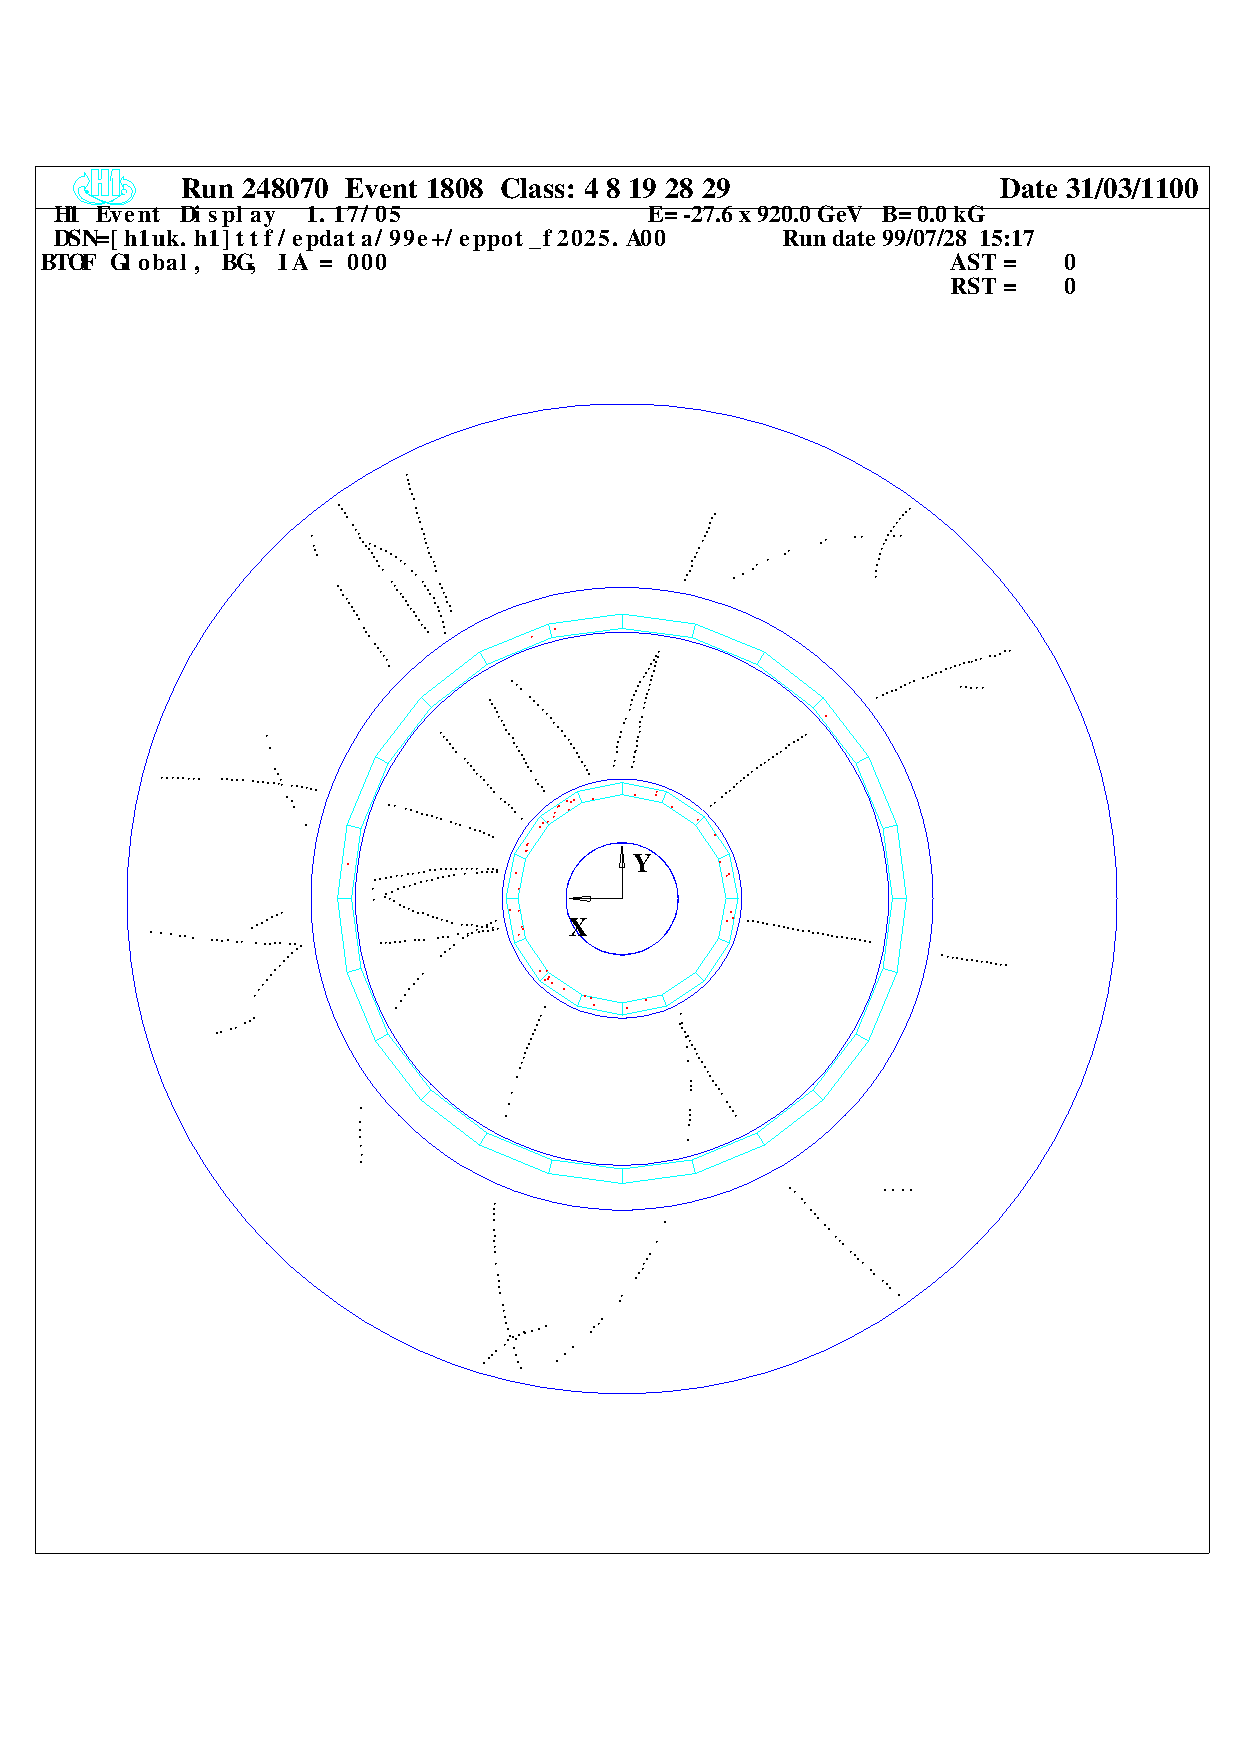
\includegraphics[width=13cm]{pics/H1}
\centering
\caption{Particle trajectories in the central drift chamber of the H1 experiment. The drift chamber is cylindrical and the anode wires are parallel to the cylindrical axis, therefore they are perpendicular to the image plane. Each point represents a wire which detected a signal. The positions are corrected by means of drift duration.}
\label{fig:H1_detector}
\end{figure}

\section{Electron drift}

The electrons released by ionization get quickly to thermal equilibrium through elastic collisions with the gas atoms. The electrons then move in arbitrary, frequently changing directions. The average kinetic energy is like in an ideal gas
\begin{equation}
< \frac{1}{2} m v^2 > = \frac{3}{2} k T.
\end{equation}
At room temperature this correlates to a velocity of \SI{120}{\kilo\meter\per\second}!

Between collisions the electrons get accelerated by the electric field over and over again. Thus the motion of the electron cloud goes along the field lines on average. 

For a start we look at a group of electrons all traveling with velocity $v$. Along a way $dx$ a fraction $N \sigma dx$ of the electrons collide with a gas atom. $N$ is the number of gas atoms per unit volume and $\sigma$ the total collision cross section. Let's call $n(t)$ the number of electrons, which didn't collide with a gas atom in a time $t$ since the last collision. Thus $n(t)$ can be calculated by
\begin{equation}
dn(t) = - N \sigma v dt = -\frac{v}{l} dt.
\label{eq:dn(t)}
\end{equation}

The quantity $l \equiv (N \sigma)^{-1}$ is called the mean free path of the electrons in the gas. Integrating (\ref{eq:dn(t)}) yields
\begin{equation}
N(t) = n_0 \exp\Big(-\frac{v}{l} t \Big).
\end{equation}

An electron experiences a constant force $e \vec{E}$ on the path between two collisions. Therefore additionally to the free movement the electron covers  the distance 
\begin{equation}
\Delta s = \frac{1}{2} \frac{eE}{m} \Delta t^2
\end{equation}
along the $\vec{E}$-field.

The mean drift velocity for electrons with velocity $v$ is thus
\begin{align*}
 v_D(v) & = \frac{\int \Delta s(t) e^{-\frac{v}{l} t}dt}{\int t e^{-\frac{v}{l}}dt} \\
 & = \frac{1}{2}\frac{eE}{m} \frac{\int t^2 e^{-\frac{v}{l} t}dt}{\int t e^{-\frac{v}{l}}dt} = \frac{eE}{m} \frac{l}{v}.
\end{align*}

In reality not all electrons are moving at the same velocity, but the velocities are distributed corresponding to the Maxwell-Boltzmann distribution. Thus to get the mean drift velocity for the whole electron cloud, one has to average over the thermal velocities. The drift velocity of the electron cloud is therefore
\begin{equation}
v_D = \frac{eE}{m} < \frac{l}{v} > = \frac{eE}{m} \tau.
\end{equation}
Where $\tau$ is the mean time between two collisions of an electron with a gas atom.

According to this simple calculation one expects the drift velocity to increase proportional to the electric field strength. For small fields this is normally the case. The proportionality constant is called the mobility.

\section{Gas Amplification}

If the accelerating electric field is strong enough, the electrons can gain enough energy between two collisions, to ionize a gas atom. The new free electrons get accelerated themselves to the point where they can ionize a gas atom and the total number of free electrons increases rapidly in a snowballing effect. 

In a constant and sufficient high electric field strength the number of secondary ionizations, which a drifting electron causes, is proportional to the covered distance. The proportionality factor $\alpha$ is called the first Townsend-coefficient. The factor is dependent on the electric field strength. One finds an empirical dependency of the form
\begin{equation}
\alpha = A \exp \Bigl( - \frac{B}{E} \Bigr),
\label{eq:townsend}
\end{equation}
with coefficients $A$ and $B$, which depend on the gas. 

Hence the total number of electrons increases along the way $dx$ by
\begin{equation}
dn = n \alpha dx.
\end{equation}
Generally the electric field, in which the gas amplification occurs, is inhomogeneous. Thus $\alpha$ becomes dependent on position. If the gas amplification starts at a distance $r_0$, the number of electrons which arrive at the signal wire (radius $r_2$) is 
\begin{equation}
n(x) = n_0 \exp \int_{r_0}^{r_2} \alpha(x) dx.
\end{equation}

In principle the characteristics of the electric field are dependent on the form and potentials of all the electrodes. But within immediate distance to the signal wires, that is for distances which are very much smaller than  the distances to the other electrodes, the field profile is always the same. For a cylindrical geometry the field strength can be described by:
\begin{equation}
E(r) = \frac{1}{r} \frac{V}{\ln (r_2/r_1)}
\end{equation}
Where $V$ is the voltage between the wire and the other electrode, which is located at radius $r_1$. From this equation one recognizes, that the field goes like $1/r$ near the wire and that with small wires one can achieve high field strengths. The signal wires in our chamber have a diameter of \SI{50}{\micro\meter}.

The gas amplification or specifically the number of electrons in the avalanche arriving at the wire is therefore
\begin{align*}
M &= \exp \Biggl\{ \int_{r_0}^{r_2} A \exp \Biggl( - B \frac{r \ln(r_2/r_1)}{V}\Biggr)\Biggr\} \\
&= \exp \Biggl[ A \frac{V}{\ln(r_2/r_1)} \exp \Biggl( - B \frac{r \ln(r_2/r_1)}{V} \Biggr) \Biggr]_{r_0}^{r_1} \\
& = \exp \Biggl[ \frac{V}{\ln(r_2/r_1)} \bigl(\alpha(r_2) - \alpha (r_0)\bigr) \Biggr]
\end{align*}

The Townsend-coefficient $\alpha(r_0)$ at the start of the avalanche is much smaller, than the one near the wire. From equation~(\ref{eq:townsend} it follows that for high enough field strengths $\alpha$ tends to a constant value and thus $\alpha(r_2) - \alpha(r_0) \approx const.$ The gas amplification is therefore  dependent on the potential of the signal wires simply by
\begin{equation}
M \propto e^V.
\end{equation}
The gas amplification increases exponentially with increasing voltage!

However this increase does not go on forever. If the charge of the  avalanche is high enough to affect the electric field, the resulting signal is no longer proportional to the originally released charge.

If the voltage gets too high, electric discharges start to occur, where permanent gas discharges take place and a very high current flows. The equipment can be damaged in this process. 

\section{Cosmic Radiation}

Particles, in particular protons, coming from the universe and from the sun constantly impact the earth. The energy of these particles ranges from $10^9$ up to $10^{20}$ \SI{}{\giga\electronvolt}. The particles loose their energy by colliding with atoms in the upper atmosphere. In this process they create jets of new particles. Many of these secondary particles collide with gas atoms themselves and only a small fraction reaches the surface of the earth.

 In the midst of these secondary particles there are also pions, which decay into muons and neutrinos after only a short amount of time. The neutral neutrinos only interact via the weak force and are practically undetectable. The charged muons loose energy due to ionization, but have cross sections for inelastic collisions with air atoms which are much smaller than the ones for the strongly interacting protons.

On the earth's surface the cosmic radiation then consists mostly of muons.

\section{Measurement Setup}

The mechanism consists of the actual drift chamber, the trigger, the electronics and a computer for data collection. Figure~\ref{fig:schema} shows a logic diagram of the setup. 

\begin{figure}[!h]
\includegraphics[width=13cm]{pics/Schema.jpg}
\centering
\caption{Logic diagram of the main parts of the measurement setup.}
\label{fig:schema}
\end{figure}

The Figures~\ref{fig:NIM_crate} through \ref{fig:distributor} shows the physical view of of some of the elements in Figure~\ref{fig:schema}. It contains the both the trigger logic units and power supplies from left to right the untis in the Figure~\ref{fig:NIM_crate} are:
\begin{itemize}
\item Lower voltage power supply for the amplifiers of the photomultipliers (PMTs)
\item Discriminator
\item Coincidence unit
\item Counter/scalar
\item Level converter (NIM to TTL)
\item High voltage power supply for cathode
\item High voltage power supply for anode (positive voltage)
\item High voltage power supply for field wires
\item Counter/scalar 
\item Delay unit
\end{itemize}

\subsection{Trigger formation}
The even trigger is formed in the following way. The muons crossing the scintillators produce photons in the scintillator. The photons are converted into electrical pulse by the PMTs futher multiplied and fed into the discriminator. The discriminator analyzers the signal and if the amplitude of the signal crosses the set threshold, it outputs a square NIM pulse. The NIM pulses from each discriminator are then fed into the coincidence unit. This unit, when the both inputs are set in an AND mode, analyzes whether or not the input pulses overlap in time. If they do, it outputs another NIM pulse, which in turn is fed into two duplicating counters. Each of the counters counts the pulses fed into it. Another output from the coincidence unit is delayed by the delay unit and converted to TTL pulse. The TTL pulse is then fed into the trigger input of the 1$^{st}$ DRS4 board. When the signal arrives there it gives the board a command to output the signals that are at the moment on the inputs of the DRS4 board to the computer screen and record them to hard disc, if the SAVE mode is activated. Another trigger output is fed into external trigger of an oscilloscope. Where one can observe the signals of the scintillators before and after they fed trough the discriminators. You are strongly encouraged to explore the setup yourself by tracing the cables. Understanding the trigger system is an important part of the lab. 

\begin{figure}[!h]
\includegraphics[width=13cm]{pics/NIM_crate.jpg}
\centering
\caption{NIM crate with the main logic and power supplies.}
\label{fig:NIM_crate}
\end{figure}

The Figures~\ref{fig:power_supply_front} and \ref{fig:distributor} show the front and the back of the high voltage power supply of the scintillator PMTs. Since the operation voltage of each PMT differs slightly. The output of the high voltage power supply if fed into the 1st input of the high voltage distributor (Fig.~\ref{fig:distributor}). The 1st and the 2nd outputs of the distributor are then supply voltage individually to the PMTs. The each output can be individually down regulated by a corresponding knob on the front panel of the distributor. IMPORTANT: The power supply requires a few seconds to warm up before the high voltage can be switched ON. After turning on the power suplly wait until the yellow/white indicator light is ON before flipping the high voltage switch to ON.

\begin{figure}
	\centering
		\begin{subfigure}[b]{0.8\textwidth}
				\includegraphics[width=1\linewidth]{pics/power_supply_distributor_front.jpg}
				\caption{}
				\label{fig:power_supply_front}
		\end{subfigure}
		\begin{subfigure}[b]{0.8\textwidth}
			\includegraphics[width=1\linewidth]{pics/distributor_back.jpg}
			\caption{}
			\label{fig:distributor}
		\end{subfigure}
\caption{The front (a)  and back (b) of the high voltage power supply and high voltage distributor for the scintillator PMTs.}
\end{figure}



\subsection{Drift Chamber}
\label{measurementsetupdriftchamber}

The drift field inside of our drift chamber is generated by two parallel electrodes, which have a distance of \SI{100}{\milli\meter}. To have a homogeneous electric field inside the drift chamber, the potential also has to increase linearly from the cathode to the anode at the edge of the drift chamber. This is approximately achieved with 9 electrodes, which are placed parallel to each other in a distance of \SI{1}{\centi\meter} and enclose the drift chamber. Their potentials are linearly graduated with a bleeder chain. The resulting electric field looks similarly to the electric field in Figure~ \ref{fig:potential}.

\begin{figure}[h]
\includegraphics[width=13cm]{pics/Potential}
\centering
\caption{Electric field lines and equipotential lines inside the drift chamber. The electrons drift from left to right, where the signal wires are.}
\label{fig:potential}
\end{figure}
 
 The Figure~\ref{fig:drift_camera_cross_section} shows a CAD cross section of the drift camera.

\begin{figure}[!h]
	\includegraphics[width=13cm]{pics/Driftkammer_Schnittbild.jpg}
	\centering
	\caption{CAD cross section of the drift camera. All the distances shown are correct. The camera there only 8 anode wires (shown as black dots on the left side on the picture). On each side of the anode wires the field wires (empty circles) are located equidistantly from each anode neighboring anode wire. The cathode plate is 94.3\,mm right of the anode wires. About 4\,mm To the left of the anode wires the ground plate is located. On the top and on the bottom of the drift volume the field plates are position at roughly equal distances.}
	\label{fig:drift_camera_cross_section}
\end{figure}

The anode wires, which produce the gas amplification, are placed \SI{5}{\milli\meter} in front of the ground plate. The sensitive region in which the particles can be detected is between those wires and the cathode and has a length of \SI{9.5}{\centi\meter}.

The 8 wires are arranged parallel to each other and  have a distance of \SI{10}{\milli\meter} between each other. Their diameter is only \SI{50}{\micro\meter}, so they can produce the needed high electric field strengths for the gas amplification. Between the anode wires there are field wires that make the electric field more even. These field wires have an own voltage supply, which can be left at zero though. 

The anode wires connected to a charge sensitive amplifier powered by the low voltage power supply, which amplifies the signal coming from the wire even further. This amplifier is mounted inside the drift chamber, at the end of each anode wire. The low voltage power supply is connected to the amplifier by three jacks at the front of the chamber and has to be turned on in order of being able to detect the signals on the anode wires. 

The drift chamber is mounted such that the wires are horizontal and the plane of the wires is vertical. The drift direction for the electrons is thus horizontal. A particle which travels vertically through the drift chamber will therefore induce a signal in all wires. Figure~\ref{fig:CAD} shows the interior of the drift chamber with the electrodes and the signal wires. 

\begin{figure}[h]
\includegraphics[width=13cm]{pics/Driftkammer_Ansicht_5.png}
\centering
\caption{A drawing of the drift chamber. One can observe the anode wires (the field wires between the anode wires are not shown), the electrodes which make a more homogeneous field and the cathode and ground plate.}
\label{fig:CAD}
\end{figure}


%\subsection{Trigger}
 %Above and below the drift chamber there is each a scintillator. The scintillators are used to trigger on a passage of a cosmic muon. The here used plastic scintillators produce very fast signals (\SI{1}{\nano\second}), which give a precise starting signal for the drift time measurement. The actual scintillators are rectangular and have a size of \SI{10}{\centi\meter} by \SI{20}{\centi\meter}. With light guide the scintillating light, produced by a muon passage through the scintillator, is transported to the photomultipliers, which then produce and amplify an electric signal. 

%The output of each photomultiplier is connected to a discriminator channel in the NIM-crate. When the photomultiplier signal surpasses a set discriminator threshold, the discriminators produce a NIM (logic) signal on the outputs. This signal can then be detected by a counter. A coincidence unit can select  the cases, where both scintillators produce a signal. This enables to trigger only particles which really fly through the drift chamber. 

%The high voltage supply for the scintillators comes from a general high voltage supply which is connected to a distributor. Channel 1 and 2 of the distributor connect each to one of the scintillators. The voltage can then be  tuned at the distributor for each scintillator separately.

\subsection{The DRS4 unit}
To process the incoming data from the signal wires, the wires are connected to DRS4 boards. These DRS4 boards were designed at the Paul Scherrer Institute and are capable of digitizing 4 channels each. Two boards are linked together to process all 8 channels. The DRS4 boards work like a digital oscilloscope. For details on the operation of the DRS4 boards please refer to the DRS4 manual \cite{DRS4_manual}.

The DRS4 unit comes with a computer program called drsosc located in \verb|~/Desktop/drs-5.0.6/|. A softlink to the executable is put in the home directory. The program can be started from the command line as follows: 

\begin{lstlisting}[language=bash]
$ ./drsosc
\end{lstlisting}

 It opens a GUI that emulates an oscilloscope interface and can display all 8 channels. The boards have a port for an external trigger which can be connected to the trigger logic. The trigger output of the first board is connected to the second board, so both boards receive the trigger at approximately the same time.

\section{Measurements}
The main goal of this experiment is to familiarize oneself with an operation of a small drift chamber and observe the tracks of the cosmic muons passing through it. Additionally you will develop your own data analysis technique using as a provided data conversion program as a starter.  You are advised to  perform the following measurements. Start with finding the  working point of the scintillators. Then study the gas amplification dependence on the anode voltage. Followed by the study of the dependence of the ion drift velocity on the cathode voltage. Finally, observe a few events and plot the muon traces. The following sections will give you some hints on how to perform the measurement. Overall you are encouraged to your own methods to measure the above parameters. However, if your methods deviate from the suggested, substantiate them by solid physical arguments. 

\subsection{Saving and analyzing data}
Save data in binary format (remember to add \verb|.dat| extension to the file name as it is not there by default) In the directory \verb|~/Software/driftchamber/code/| there is a program which reads the binary datafile and makes numpy arrays for each event. Please NOTE that the extantions to the analysis code  should be written by you!
%The program also outputs a file in a root format \cite{root_website}. 

\subsection{Finding the working point of the scintillators}
To get a good trigger signal you first have to find the working point of the two scintillators. For any given discriminator threshold the scintillator has a specific voltage, where all incoming signals get detected, but the voltage isn't high enough to detect too much background noise. This manifests itself in a plateau in the counts per second around this working point. You apply a voltage of about \SI{2}{\kilo\volt} on the scintillators and put one of them to "and" on the coincidence unit. Then you regulate the threshold so that there are a few counts per second. The threshold voltage can be measured with the external voltmeter. Now you have to count the triggered signals and calculate the number of counts per second for different applied voltages from around \SI{1.9}{\kilo\volt} to \SI{2.1}{\kilo\volt}. Plot the counts per second against the voltage and you will see a plateau. The working point of the scintillator is the highest voltage of the plateau. Repeat the measurement for the second scintillator. The working points of the scintillators do not have to be at the same voltage, but double check if the plateaus are at the same number of counts per second.

%\subsection{Coincidence unit} 
%Now set the scintillators to their working point and put both of them to "and" on the coincidence unit, such that it only counts the particles, which pass through both scintillators. In order to insure that the coincidence between the scintillators works correctly, measure the counts per second for different distances between the scintillators and plot them in a graph.

\subsection{Purifying the gas}
The experiment is performed at an atmospheric pressure. The gas inside the chamber is a mixture of argon and methane (50:50). It is supplied from the pressurized gas cylinder marked A on Figure~\ref{fig:gas}. The chamber is also connected to a pressure pump (D), which can evacuate the chamber. In order to evacuate the chamber the valve at the chamber to the pump (B) and the valve at the pump itself both should be opened. While the valve to the gas cyllinder (C) should be closed. The filling of the chamber is performed by closing the valves (B) and (D) and openning valves (A) and (C). Before starting  the experiment it is wise to empty the chamber and fill it up again several times, to make sure the gas inside the chamber is pure enough. The pressure inside the chamber should be at or slightly above  \SI{1}{\bar} in the end. IMPORTANT: When you finish purifying the gas inside the chamber make sure that the valve (A) on the gas cyllinder is closed.

\begin{figure}[!h]
	\includegraphics[width=12cm]{pics/valve}
	\centering
	\caption{To evacuate the chamber turn on the pump under the table and open valve D and B. Do open valve B gently, such that the pressure doesn't decrease too fast otherwise it will start to smell inside the room.  To stop evacuating first close valve B and then D. To fill the chamber with gas, first open valve A and then gently open valve C until the desired pressure is achieved. Afterwards close valve C and A.}
	\label{fig:gas}
\end{figure}

\subsection{Gas Amplification}
In the next part you want to find the optimum anode voltage amplifies that provides the maximum amplification while keeping the frequency of the sparking (electrostatic discharge) inside the chamber low. 

In order to have a high enough count rate, a  \isotope[90]{Sr}-probe can be put in the window on top of the drift chamber. This isotope decays in a $\beta$-decay into \isotope[90]{Y}, which is also a $\beta$-emitter. The electrons from the $\beta$-decays have a wide spectrum up to a maximum energy of \SI{2.28}{\mega\electronvolt}. The scintillators and the metal wall of the drift chamber stop these low-energy electrons, which is why the source has to be placed on the window and the DRS4 board should be set to trigger on one of the channels.

% Then find the lowest anode voltage at which you can see triggered signals on the oscilloscope. Set the trigger as low as possible, but high enough that the noise does not trigger the oscilloscope. With the oscilloscope you can take the mean over several pulses. Then the average pulse amplitude can be read. It is important to set the threshold of the trigger as low as possible, because a trigger which is set too high can falsify the average signal amplitude.

Then you have to repeat the measurement for increasing anode voltages and plot the average pulse amplitude against the anode voltage. Be careful with increasing the voltage, because the actual voltage follows the adjusted value with some delay. Increase the voltage only in small steps and wait until it stabilizes. If you see a breakdown on the oscilloscope, immediately decrease the anode voltage. Figure~\ref{fig:breakdown} shows how a typical breakdown looks like on the oscilloscope. Do not increase the anode voltage over \SI{4}{\kilo\volt}. 

\begin{figure}[h]
\includegraphics[width=10cm]{pics/breakdown}
\centering
\caption{A picture of a typical display of an oscilloscope at the time of a breakdown. The anode voltage inside the drift chamber gets too high and electric discharge occurs, which produces this signal. If a breakdown is visible or audible inside the chamber, the anode voltage has to be decreased immediately.}
\label{fig:breakdown}
\end{figure}

\subsection{Drift Velocity}
Now set the anode voltage to the optimal value, which was determined in the previous task. Because we now want to make a time measurement, the external trigger should be used. The scintillators must be placed above and below the drift chamber. The scintillators should be positioned exactly vertically above each other. In oder to find the time electron needs to travel through the whole chamber (94.3 mm) to the anode wire.The events with the earliest signals (muon passes next to the anode wire) and the latest signals (muon passes next to the cathode plate) should be observed. Note that because of the geometrical acceptance of the scintillator triger, such events have very low probability. (You are encouraged to estimate this probability). Therefore a significant ammount of events ($\sim$10000) should be recorded. Since the rate of the muons is low, this measurements should be run overnight.

 With the assumption of a constant velocity you can then derive the drift velocity. Repeat this measurement for several cathode voltages between \SI{500}{\volt} and \SI{4000}{\volt} to see how the drift velocity depends on the cathode voltage. The exact ammount of points you chose will depend on your time and curiousity.

\subsection{Muon tracking}

Now you have all the data to track the muons. You can either collect a small ammount data at you favourite settings or use a sample of the data from the drift velocity measurements.  The drift velocity will help you to compute the distance at which the muon passed the signal wire. Then using the vertical positions wires plot the trajectories.

\bibliographystyle{unsrt}
\bibliography{driftchamber_references}

\pagebreak

\appendix
\section{Sample Analysis Code:}

The latest analysis code is located at:

\url{https://github.com/dmitryhits/driftchamber/blob/master/code/decode.py}

Note that at the moment this is the only program that works, but you are encouraged to make others working as well.


\lstinputlisting[language=Python]{decode.py}

\end{document}
